\label{sec:Introduction}
\begin{figure*}
	\centering
		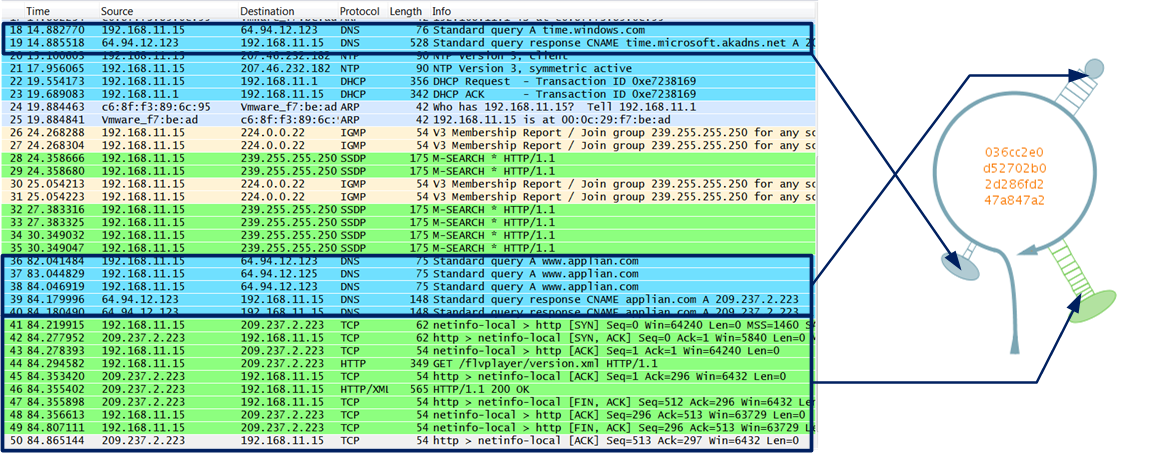
\includegraphics[width=0.78\linewidth]{pics/Mapping.png}
	\label{fig:Mapping}
	\caption{We illustrate our mapping scheme by a simple example network traces generated by malware instance~(036cc2e0): there are three streams of packets~(as highlighted by rectangles in the flow records produced by Wireshark~\cite{Wireshark}) are mapped to three cilia in the cell view on the right. The user can select a cilium for detailed information about the stream.}
\end{figure*}


Malware remains at the forefront of most security threats on the Internet. Nearly every existing malware instance relies on network communication to facilitate its attacks, such as communicating with its command and control (C$\&$C) server, sending spam emails or operating in a fast-flux service net-work. Therefore, the set of network traces are commonly used to characterize a malware sample's behavior. As an essential technology that combats illegal income for the attackers, malware analysis has been playing a crucial role in supplying signatures to investigation and detection systems. 

There is a growing need for visual presentations in the workplace of malware analysis: new instances of ``in the wild'' malware samples are collected daily. In a typical analysis scenario, each malware instance is run on a controlled environment where its host-level and network-level activities are captured as host and network traces. In order to keep track of each sample, security researchers maintain large databases of network traces. Due to their sheer size, it is a daunting task to look into the details of each sample.

Current malware analysis approaches pose several challenges to the analytic process itself which complicate visualization design. First, the network traces generated from the controlled environment contain information irrelevant to understanding most malware's behavior (e.g. DHCP, ARP, SSDP packets and local host IP).The ambition to visualize them all not only complicates the design, but also causes confusion to the analysts. Since many of these are known a priori, we filter irrelevant attributes during preprocessing. Second, even though we have discarded the irrelevant content, the analyst can easily lose the big picture of malware activities by focusing on individual packets. To handle this, we aggregate packets into streams separated by protocol. Specifically, we focus on DNS and TCP streams as they are often used by malware for communication. Third, each stream can have drastically different numbers of packets and such an uneven distribution presents in nearly every attribute space (e.g. total size of transmission, starting time, duration). Linearly mapping these attributes not only consumes screen real-estate, but also draws the viewer's attention away from those small but potentially important streams. Last, but most importantly, showing all relevant attributes in a single view, a vivid graphical representation of individual malware behaviors, requires an original design. In the absence of an intuitive presentation of the set of network traces, malware behavior analysis can still be tedious.     

The goal of this paper is to present a visualization system and a model design that address the above challenges. Our work claims the following contributions:
\begin{itemize}

	\item \textbf{Data collection and preprocessing.} As explained earlier, the malware network traces were captured by packet sniffer software in a controlled environment. The preprocessing consists of two steps: \emph{pruning} and \emph{bundling}. The raw network data are pruned by preserving protocols known to be used commonly by malware seen in the wild. Then we bundle the packets according to their protocols and hosts so that each stream of communications is semantically clear.  
		
	\item \textbf{Interface and visualization metaphor.} We design a intuitive view, which we call the \emph{cell view}, to represent a set of streams generated by any malware instance. A cell view consists of a \emph{circular timeline}, a \emph{disk panel} to display details-on-demand, and a set of \emph{cilia} oriented clockwise along the timeline to represent the set of streams. This metaphorical structure allows the viewer to select and compare among streams as well as among malware instances.    
		     
	\item \textbf{Mapping and layout techniques for sparsely distributed attributes.} As explained earlier, the majority of the communication~(in terms of the number of packets, transmission size) takes place within a small percentage of streams. Also, many streams may occur within a short period of time. To cope with these uneven distributions, we use geometric sequence and inverse logarithm to map discrete or continuous attribute values. We also present a recursive angle mapping algorithm that help to produce equalized layout for viewing streams that are cluttered over time.          
\end{itemize}

This paper is organized as follows. Sec.~\ref{sec:prior} introduces several related security visualization systems. Sec.~\ref{sec:overview} presents an expository account of malware analysis infrastructure for the benefit of readers who are not familiar with the technique. We then introduce our design and implementation in Sec.\ref{sec:implementation}. We apply the visualization model to a corpus of real-world malware samples and Sec.~\ref{sec:interaction} introduces user interaction scenarios with different components of MalwareVis. Finally, Sec.~\ref{sec:discuss} discusses and reflects on the project process; Sec.~\ref{sec:conclude} concludes the paper.  




